\documentclass{standalone}
\usepackage{tikz}
\usetikzlibrary{3d}
\begin{document}%
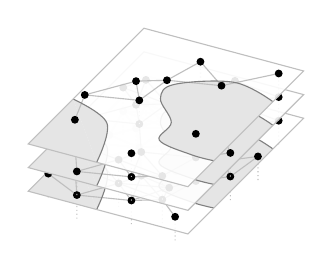
\begin{tikzpicture}

   \begin{scope}[x  = {(-0.15cm,-0.15cm)},
                       y  = {(0.2898cm,-0.0776cm)},
                       z  = {(0cm,0.30cm)},
                       scale = 2,
                       color = {lightgray}]

   % under bottom face ...
   \begin{scope}[canvas is xy plane at z=-0.5]

      % graph!
      % (same as below)
      % $ rosrun ompl_lemur generate-roadmap --dim=2 --bounds=0:0,4.9 --bounds=1:0,3.5 --roadmap-type=Halton --roadmap-param=num=30 --roadmap-param=radius=1.0 --num-batches=1 --out-file=blah.graphio --out-format=graphio
      \coordinate (uv0) at (2.45,1.1666666666666665);
      \coordinate (uv1) at (1.225,2.333333333333333);
      \coordinate (uv2) at (3.6750000000000003,0.38888888888888884);
      \coordinate (uv3) at (0.6125,1.5555555555555554);
      \coordinate (uv4) at (3.0625,2.722222222222222);
      \coordinate (uv5) at (1.8375000000000001,0.7777777777777777);
      \coordinate (uv6) at (4.2875000000000005,1.9444444444444446);
      \coordinate (uv7) at (0.30625,3.1111111111111107);
      \coordinate (uv8) at (2.75625,0.12962962962962962);
      \coordinate (uv9) at (1.53125,1.2962962962962963);
      \coordinate (uv10) at (3.98125,2.462962962962963);
      \coordinate (uv11) at (0.9187500000000001,0.5185185185185185);
      \coordinate (uv12) at (3.3687500000000004,1.6851851851851851);
      \coordinate (uv13) at (2.1437500000000003,2.851851851851851);
      \coordinate (uv14) at (4.59375,0.9074074074074073);
      \coordinate (uv15) at (0.153125,2.074074074074074);
      \coordinate (uv16) at (2.6031250000000004,3.2407407407407405);
      \coordinate (uv17) at (1.378125,0.25925925925925924);
      \coordinate (uv18) at (3.8281250000000004,1.4259259259259258);
      \coordinate (uv19) at (0.765625,2.5925925925925926);
      \coordinate (uv20) at (3.215625,0.6481481481481481);
      \coordinate (uv21) at (1.990625,1.8148148148148147);
      \coordinate (uv22) at (4.440625000000001,2.981481481481481);
      \coordinate (uv23) at (0.45937500000000003,1.037037037037037);
      \coordinate (uv24) at (2.9093750000000003,2.2037037037037037);
      \coordinate (uv25) at (1.6843750000000002,3.3703703703703702);
      \coordinate (uv26) at (4.134375,0.043209876543209874);
      \coordinate (uv27) at (1.0718750000000001,1.2098765432098766);
      \coordinate (uv28) at (3.521875,2.3765432098765427);
      \coordinate (uv29) at (2.296875,0.43209876543209874);

   \end{scope}
   
   % bottom face
   \begin{scope}[canvas is xy plane at z=0]

      % graph!
      % $ rosrun ompl_lemur generate-roadmap --dim=2 --bounds=0:0,4.9 --bounds=1:0,3.5 --roadmap-type=Halton --roadmap-param=num=30 --roadmap-param=radius=1.0 --num-batches=1 --out-file=blah.graphio --out-format=graphio
      \coordinate (bv0) at (2.45,1.1666666666666665);
      \coordinate (bv1) at (1.225,2.333333333333333);
      \coordinate (bv2) at (3.6750000000000003,0.38888888888888884);
      \coordinate (bv3) at (0.6125,1.5555555555555554);
      \coordinate (bv4) at (3.0625,2.722222222222222);
      \coordinate (bv5) at (1.8375000000000001,0.7777777777777777);
      \coordinate (bv6) at (4.2875000000000005,1.9444444444444446);
      \coordinate (bv7) at (0.30625,3.1111111111111107);
      \coordinate (bv8) at (2.75625,0.12962962962962962);
      \coordinate (bv9) at (1.53125,1.2962962962962963);
      \coordinate (bv10) at (3.98125,2.462962962962963);
      \coordinate (bv11) at (0.9187500000000001,0.5185185185185185);
      \coordinate (bv12) at (3.3687500000000004,1.6851851851851851);
      \coordinate (bv13) at (2.1437500000000003,2.851851851851851);
      \coordinate (bv14) at (4.59375,0.9074074074074073);
      \coordinate (bv15) at (0.153125,2.074074074074074);
      \coordinate (bv16) at (2.6031250000000004,3.2407407407407405);
      \coordinate (bv17) at (1.378125,0.25925925925925924);
      \coordinate (bv18) at (3.8281250000000004,1.4259259259259258);
      \coordinate (bv19) at (0.765625,2.5925925925925926);
      \coordinate (bv20) at (3.215625,0.6481481481481481);
      \coordinate (bv21) at (1.990625,1.8148148148148147);
      \coordinate (bv22) at (4.440625000000001,2.981481481481481);
      \coordinate (bv23) at (0.45937500000000003,1.037037037037037);
      \coordinate (bv24) at (2.9093750000000003,2.2037037037037037);
      \coordinate (bv25) at (1.6843750000000002,3.3703703703703702);
      \coordinate (bv26) at (4.134375,0.043209876543209874);
      \coordinate (bv27) at (1.0718750000000001,1.2098765432098766);
      \coordinate (bv28) at (3.521875,2.3765432098765427);
      \coordinate (bv29) at (2.296875,0.43209876543209874);

      % edges from under
      \draw[densely dotted] (uv0)  -- (bv0);
      \draw[densely dotted] (uv1)  -- (bv1);
      \draw[densely dotted] (uv2)  -- (bv2);
      \draw[densely dotted] (uv3)  -- (bv3);
      \draw[densely dotted] (uv4)  -- (bv4);
      \draw[densely dotted] (uv5)  -- (bv5);
      \draw[densely dotted] (uv6)  -- (bv6);
      \draw[densely dotted] (uv7)  -- (bv7);
      \draw[densely dotted] (uv8)  -- (bv8);
      \draw[densely dotted] (uv9)  -- (bv9);
      \draw[densely dotted] (uv10) -- (bv10);
      \draw[densely dotted] (uv11) -- (bv11);
      \draw[densely dotted] (uv12) -- (bv12);
      \draw[densely dotted] (uv13) -- (bv13);
      \draw[densely dotted] (uv14) -- (bv14);
      \draw[densely dotted] (uv15) -- (bv15);
      \draw[densely dotted] (uv16) -- (bv16);
      \draw[densely dotted] (uv17) -- (bv17);
      \draw[densely dotted] (uv18) -- (bv18);
      \draw[densely dotted] (uv19) -- (bv19);
      \draw[densely dotted] (uv20) -- (bv20);
      \draw[densely dotted] (uv21) -- (bv21);
      \draw[densely dotted] (uv22) -- (bv22);
      \draw[densely dotted] (uv23) -- (bv23);
      \draw[densely dotted] (uv24) -- (bv24);
      \draw[densely dotted] (uv25) -- (bv25);
      \draw[densely dotted] (uv26) -- (bv26);
      \draw[densely dotted] (uv27) -- (bv27);
      \draw[densely dotted] (uv28) -- (bv28);
      \draw[densely dotted] (uv29) -- (bv29);

      \fill[color=white,opacity=0.9] (0,0) -- (0,3.5) -- (4.9,3.5) -- (4.9,0) -- cycle;

      % obstacle 1 fill
      \fill[black!10] plot [smooth,tension=0.6] coordinates {
         (1.3,3.5) (1.0,2.5) (1.6,1.5) (2.2,1.5)
         (2.9,2.1) (3.6,2.2) (3.8,3.0) (3.8,3.5)};

      % obstacle 2 fill
      \fill[black!10] plot [smooth,tension=0.6] coordinates {
         (3.0,0.0) (3.5,1.0) (4.9,1.5)};
      \fill[black!10] (4.9,1.5) -- (4.9,0.0) -- (3.0,0.0) -- cycle;
      
      \draw (bv3) -- (bv1);
      \draw (bv5) -- (bv0);
      \draw (bv7) -- (bv1);
      \draw (bv8) -- (bv0);
      \draw (bv8) -- (bv2);
      \draw (bv8) -- (bv5);
      \draw (bv9) -- (bv0);
      \draw (bv9) -- (bv1);
      \draw (bv9) -- (bv3);
      \draw (bv9) -- (bv5);
      \draw (bv10) -- (bv4);
      \draw (bv10) -- (bv6);
      \draw (bv11) -- (bv3);
      \draw (bv11) -- (bv5);
      \draw (bv11) -- (bv9);
      \draw (bv12) -- (bv0);
      \draw (bv12) -- (bv4);
      \draw (bv12) -- (bv6);
      \draw (bv12) -- (bv10);
      \draw (bv13) -- (bv1);
      \draw (bv13) -- (bv4);
      \draw (bv14) -- (bv2);
      \draw (bv14) -- (bv6);
      \draw (bv15) -- (bv1);
      \draw (bv15) -- (bv3);
      \draw (bv15) -- (bv7);
      \draw (bv16) -- (bv4);
      \draw (bv16) -- (bv13);
      \draw (bv17) -- (bv5);
      \draw (bv17) -- (bv9);
      \draw (bv17) -- (bv11);
      \draw (bv18) -- (bv2);
      \draw (bv18) -- (bv6);
      \draw (bv18) -- (bv10);
      \draw (bv18) -- (bv12);
      \draw (bv18) -- (bv14);
      \draw (bv19) -- (bv1);
      \draw (bv19) -- (bv3);
      \draw (bv19) -- (bv7);
      \draw (bv19) -- (bv15);
      \draw (bv20) -- (bv0);
      \draw (bv20) -- (bv2);
      \draw (bv20) -- (bv8);
      \draw (bv20) -- (bv18);
      \draw (bv21) -- (bv0);
      \draw (bv21) -- (bv1);
      \draw (bv21) -- (bv9);
      \draw (bv22) -- (bv10);
      \draw (bv23) -- (bv3);
      \draw (bv23) -- (bv11);
      \draw (bv24) -- (bv4);
      \draw (bv24) -- (bv12);
      \draw (bv24) -- (bv21);
      \draw (bv25) -- (bv13);
      \draw (bv25) -- (bv16);
      \draw (bv26) -- (bv2);
      \draw (bv26) -- (bv14);
      \draw (bv27) -- (bv3);
      \draw (bv27) -- (bv5);
      \draw (bv27) -- (bv9);
      \draw (bv27) -- (bv11);
      \draw (bv27) -- (bv17);
      \draw (bv27) -- (bv23);
      \draw (bv28) -- (bv4);
      \draw (bv28) -- (bv6);
      \draw (bv28) -- (bv10);
      \draw (bv28) -- (bv12);
      \draw (bv28) -- (bv18);
      \draw (bv28) -- (bv24);
      \draw (bv29) -- (bv0);
      \draw (bv29) -- (bv5);
      \draw (bv29) -- (bv8);
      \draw (bv29) -- (bv17);
      \draw (bv29) -- (bv20);

      % obstacle 1 boundary
      \draw[black!50] plot [smooth,tension=0.6] coordinates {
         (1.3,3.5) (1.0,2.5) (1.6,1.5) (2.2,1.5)
         (2.9,2.1) (3.6,2.2) (3.8,3.0) (3.8,3.5)};

      % obstacle 2 boundary
      \draw[black!50] plot [smooth,tension=0.6] coordinates {
         (3.0,0.0) (3.5,1.0) (4.9,1.5)};

      % path
      %\draw plot [smooth,tension=0.6,thick] coordinates {
      %   (0.5,2.0) (1.0,1.0) (2.8,1.0) (4.0,1.9) (4.4,2.2)};

      % path endpoints / labels
      %\fill[black] (0.5,2.0) circle (0.05cm);
      %\fill[black] (4.4,2.2) circle (0.05cm);
      
      % C-space border
      \draw (0,0) -- (0,3.5) -- (4.9,3.5) -- (4.9,0) -- cycle;

      % nodes
      \node[inner sep=1pt,fill=black,circle] at (bv0) {};
      \node[inner sep=1pt,fill=black,circle] at (bv1) {};
      \node[inner sep=1pt,fill=black,circle] at (bv2) {};
      \node[inner sep=1pt,fill=black,circle] at (bv3) {};
      \node[inner sep=1pt,fill=black,circle] at (bv4) {};
      \node[inner sep=1pt,fill=black,circle] at (bv5) {};
      \node[inner sep=1pt,fill=black,circle] at (bv6) {};
      \node[inner sep=1pt,fill=black,circle] at (bv7) {};
      \node[inner sep=1pt,fill=black,circle] at (bv8) {};
      \node[inner sep=1pt,fill=black,circle] at (bv9) {};
      \node[inner sep=1pt,fill=black,circle] at (bv10) {};
      \node[inner sep=1pt,fill=black,circle] at (bv11) {};
      \node[inner sep=1pt,fill=black,circle] at (bv12) {};
      \node[inner sep=1pt,fill=black,circle] at (bv13) {};
      \node[inner sep=1pt,fill=black,circle] at (bv14) {};
      \node[inner sep=1pt,fill=black,circle] at (bv15) {};
      \node[inner sep=1pt,fill=black,circle] at (bv16) {};
      \node[inner sep=1pt,fill=black,circle] at (bv17) {};
      \node[inner sep=1pt,fill=black,circle] at (bv18) {};
      \node[inner sep=1pt,fill=black,circle] at (bv19) {};
      \node[inner sep=1pt,fill=black,circle] at (bv20) {};
      \node[inner sep=1pt,fill=black,circle] at (bv21) {};
      \node[inner sep=1pt,fill=black,circle] at (bv22) {};
      \node[inner sep=1pt,fill=black,circle] at (bv23) {};
      \node[inner sep=1pt,fill=black,circle] at (bv24) {};
      \node[inner sep=1pt,fill=black,circle] at (bv25) {};
      \node[inner sep=1pt,fill=black,circle] at (bv26) {};
      \node[inner sep=1pt,fill=black,circle] at (bv27) {};
      \node[inner sep=1pt,fill=black,circle] at (bv28) {};
      \node[inner sep=1pt,fill=black,circle] at (bv29) {};
      
   \end{scope}
   
   
   
   % middle face
   \begin{scope}[canvas is xy plane at z=0.5]

      % $ rosrun ompl_lemur generate-roadmap --dim=2 --bounds=0:0,4.9 --bounds=1:0,3.5 --roadmap-type=Halton --roadmap-param=num=20 --roadmap-param=radius=1.2 --num-batches=1 --out-file=blah.graphio --out-format=graphio
      \coordinate (mv0) at (2.45,1.1666666666666665);
      \coordinate (mv1) at (1.225,2.333333333333333);
      \coordinate (mv2) at (3.6750000000000003,0.38888888888888884);
      \coordinate (mv3) at (0.6125,1.5555555555555554);
      \coordinate (mv4) at (3.0625,2.722222222222222);
      \coordinate (mv5) at (1.8375000000000001,0.7777777777777777);
      \coordinate (mv6) at (4.2875000000000005,1.9444444444444446);
      \coordinate (mv7) at (0.30625,3.1111111111111107);
      \coordinate (mv8) at (2.75625,0.12962962962962962);
      \coordinate (mv9) at (1.53125,1.2962962962962963);
      \coordinate (mv10) at (3.98125,2.462962962962963);
      \coordinate (mv11) at (0.9187500000000001,0.5185185185185185);
      \coordinate (mv12) at (3.3687500000000004,1.6851851851851851);
      \coordinate (mv13) at (2.1437500000000003,2.851851851851851);
      \coordinate (mv14) at (4.59375,0.9074074074074073);
      \coordinate (mv15) at (0.153125,2.074074074074074);
      \coordinate (mv16) at (2.6031250000000004,3.2407407407407405);
      \coordinate (mv17) at (1.378125,0.25925925925925924);
      \coordinate (mv18) at (3.8281250000000004,1.4259259259259258);
      \coordinate (mv19) at (0.765625,2.5925925925925926);

      % edges from bottom
      \draw[densely dotted] (bv0)  -- (mv0);
      \draw[densely dotted] (bv1)  -- (mv1);
      \draw[densely dotted] (bv2)  -- (mv2);
      \draw[densely dotted] (bv3)  -- (mv3);
      \draw[densely dotted] (bv4)  -- (mv4);
      \draw[densely dotted] (bv5)  -- (mv5);
      \draw[densely dotted] (bv6)  -- (mv6);
      \draw[densely dotted] (bv7)  -- (mv7);
      \draw[densely dotted] (bv8)  -- (mv8);
      \draw[densely dotted] (bv9)  -- (mv9);
      \draw[densely dotted] (bv10) -- (mv10);
      \draw[densely dotted] (bv11) -- (mv11);
      \draw[densely dotted] (bv12) -- (mv12);
      \draw[densely dotted] (bv13) -- (mv13);
      \draw[densely dotted] (bv14) -- (mv14);
      \draw[densely dotted] (bv15) -- (mv15);
      \draw[densely dotted] (bv16) -- (mv16);
      \draw[densely dotted] (bv17) -- (mv17);
      \draw[densely dotted] (bv18) -- (mv18);
      \draw[densely dotted] (bv19) -- (mv19);

      \fill[color=white,opacity=0.9] (0,0) -- (0,3.5) -- (4.9,3.5) -- (4.9,0) -- cycle;

      % obstacle 1 fill
      \fill[black!10] plot [smooth,tension=0.6] coordinates {
         (1.3,3.5) (1.0,2.5) (1.6,1.5) (2.2,1.5)
         (2.9,2.1) (3.6,2.2) (3.8,3.0) (3.8,3.5)};
      % obstacle 2 fill
      \fill[black!10] plot [smooth,tension=0.6] coordinates {
         (3.0,0.0) (3.5,1.0) (4.9,1.5)};
      \fill[black!10] (4.9,1.5) -- (4.9,0.0) -- (3.0,0.0) -- cycle;

      % intra-middle edges
      \draw (mv3) -- (mv1);
      \draw (mv5) -- (mv0);
      \draw (mv7) -- (mv1);
      \draw (mv8) -- (mv0);
      \draw (mv8) -- (mv2);
      \draw (mv8) -- (mv5);
      \draw (mv9) -- (mv0);
      \draw (mv9) -- (mv1);
      \draw (mv9) -- (mv3);
      \draw (mv9) -- (mv5);
      \draw (mv10) -- (mv4);
      \draw (mv10) -- (mv6);
      \draw (mv11) -- (mv3);
      \draw (mv11) -- (mv5);
      \draw (mv11) -- (mv9);
      \draw (mv12) -- (mv0);
      \draw (mv12) -- (mv4);
      \draw (mv12) -- (mv6);
      \draw (mv12) -- (mv10);
      \draw (mv13) -- (mv1);
      \draw (mv13) -- (mv4);
      \draw (mv14) -- (mv2);
      \draw (mv14) -- (mv6);
      \draw (mv15) -- (mv1);
      \draw (mv15) -- (mv3);
      \draw (mv15) -- (mv7);
      \draw (mv16) -- (mv4);
      \draw (mv16) -- (mv13);
      \draw (mv17) -- (mv5);
      \draw (mv17) -- (mv9);
      \draw (mv17) -- (mv11);
      \draw (mv18) -- (mv2);
      \draw (mv18) -- (mv6);
      \draw (mv18) -- (mv10);
      \draw (mv18) -- (mv12);
      \draw (mv18) -- (mv14);
      \draw (mv19) -- (mv1);
      \draw (mv19) -- (mv3);
      \draw (mv19) -- (mv7);
      \draw (mv19) -- (mv15);

      % nodes
      \node[inner sep=1pt,fill=black,circle] at (mv0) {};
      \node[inner sep=1pt,fill=black,circle] at (mv1) {};
      \node[inner sep=1pt,fill=black,circle] at (mv2) {};
      \node[inner sep=1pt,fill=black,circle] at (mv3) {};
      \node[inner sep=1pt,fill=black,circle] at (mv4) {};
      \node[inner sep=1pt,fill=black,circle] at (mv5) {};
      \node[inner sep=1pt,fill=black,circle] at (mv6) {};
      \node[inner sep=1pt,fill=black,circle] at (mv7) {};
      \node[inner sep=1pt,fill=black,circle] at (mv8) {};
      \node[inner sep=1pt,fill=black,circle] at (mv9) {};
      \node[inner sep=1pt,fill=black,circle] at (mv10) {};
      \node[inner sep=1pt,fill=black,circle] at (mv11) {};
      \node[inner sep=1pt,fill=black,circle] at (mv12) {};
      \node[inner sep=1pt,fill=black,circle] at (mv13) {};
      \node[inner sep=1pt,fill=black,circle] at (mv14) {};
      \node[inner sep=1pt,fill=black,circle] at (mv15) {};
      \node[inner sep=1pt,fill=black,circle] at (mv16) {};
      \node[inner sep=1pt,fill=black,circle] at (mv17) {};
      \node[inner sep=1pt,fill=black,circle] at (mv18) {};
      \node[inner sep=1pt,fill=black,circle] at (mv19) {};

      % obstacle 1 boundary
      \draw[black!50] plot [smooth,tension=0.6] coordinates {
         (1.3,3.5) (1.0,2.5) (1.6,1.5) (2.2,1.5)
         (2.9,2.1) (3.6,2.2) (3.8,3.0) (3.8,3.5)};

      % obstacle 2 boundary
      \draw[black!50] plot [smooth,tension=0.6] coordinates {
         (3.0,0.0) (3.5,1.0) (4.9,1.5)};

      % path
      %\draw plot [smooth,tension=0.6,thick] coordinates {
      %   (0.5,2.0) (1.0,1.0) (2.8,1.0) (4.0,1.9) (4.4,2.2)};

      % path endpoints / labels
      %\fill[black] (0.5,2.0) circle (0.05cm);
      %\fill[black] (4.4,2.2) circle (0.05cm);
      
      % C-space border
      \draw (0,0) -- (0,3.5) -- (4.9,3.5) -- (4.9,0) -- cycle;
      
   \end{scope}
   
   
   % top face
   \begin{scope}[canvas is xy plane at z=1.0]

      % $ rosrun ompl_lemur generate-roadmap --dim=2 --bounds=0:0,4.9 --bounds=1:0,3.5 --roadmap-type=Halton --roadmap-param=num=10 --roadmap-param=radius=1.4 --num-batches=1 --out-file=blah.graphio --out-format=graphio
      \coordinate (tv0) at (2.45,1.1666666666666665);
      \coordinate (tv1) at (1.225,2.333333333333333);
      \coordinate (tv2) at (3.6750000000000003,0.38888888888888884);
      \coordinate (tv3) at (0.6125,1.5555555555555554);
      \coordinate (tv4) at (3.0625,2.722222222222222);
      \coordinate (tv5) at (1.8375000000000001,0.7777777777777777);
      \coordinate (tv6) at (4.2875000000000005,1.9444444444444446);
      \coordinate (tv7) at (0.30625,3.1111111111111107);
      \coordinate (tv8) at (2.75625,0.12962962962962962);
      \coordinate (tv9) at (1.53125,1.2962962962962963);

      % edges from middle
      \draw[densely dotted] (mv0)  -- (tv0);
      \draw[densely dotted] (mv1)  -- (tv1);
      \draw[densely dotted] (mv2)  -- (tv2);
      \draw[densely dotted] (mv3)  -- (tv3);
      \draw[densely dotted] (mv4)  -- (tv4);
      \draw[densely dotted] (mv5)  -- (tv5);
      \draw[densely dotted] (mv6)  -- (tv6);
      \draw[densely dotted] (mv7)  -- (tv7);
      \draw[densely dotted] (mv8)  -- (tv8);
      \draw[densely dotted] (mv9)  -- (tv9);

      \fill[color=white,opacity=0.9] (0,0) -- (0,3.5) -- (4.9,3.5) -- (4.9,0) -- cycle;
      
      % obstacle 1 fill
      \fill[black!10] plot [smooth,tension=0.6] coordinates {
         (1.3,3.5) (1.0,2.5) (1.6,1.5) (2.2,1.5)
         (2.9,2.1) (3.6,2.2) (3.8,3.0) (3.8,3.5)};
      % obstacle 2 fill
      \fill[black!10] plot [smooth,tension=0.6] coordinates {
         (3.0,0.0) (3.5,1.0) (4.9,1.5)};
      \fill[black!10] (4.9,1.5) -- (4.9,0.0) -- (3.0,0.0) -- cycle;

      % inter edges
      \draw (tv3) -- (tv1);
      \draw (tv5) -- (tv0);
      \draw (tv7) -- (tv1);
      \draw (tv8) -- (tv0);
      \draw (tv8) -- (tv2);
      \draw (tv8) -- (tv5);
      \draw (tv9) -- (tv0);
      \draw (tv9) -- (tv1);
      \draw (tv9) -- (tv3);
      \draw (tv9) -- (tv5);

      % nodes
      \node[inner sep=1pt,fill=black,circle] at (tv0) {};
      \node[inner sep=1pt,fill=black,circle] at (tv1) {};
      \node[inner sep=1pt,fill=black,circle] at (tv2) {};
      \node[inner sep=1pt,fill=black,circle] at (tv3) {};
      \node[inner sep=1pt,fill=black,circle] at (tv4) {};
      \node[inner sep=1pt,fill=black,circle] at (tv5) {};
      \node[inner sep=1pt,fill=black,circle] at (tv6) {};
      \node[inner sep=1pt,fill=black,circle] at (tv7) {};
      \node[inner sep=1pt,fill=black,circle] at (tv8) {};
      \node[inner sep=1pt,fill=black,circle] at (tv9) {};
      
      % obstacle 1 boundary
      \draw[black!50] plot [smooth,tension=0.6] coordinates {
         (1.3,3.5) (1.0,2.5) (1.6,1.5) (2.2,1.5)
         (2.9,2.1) (3.6,2.2) (3.8,3.0) (3.8,3.5)};
      % obstacle 2 boundary
      \draw[black!50] plot [smooth,tension=0.6] coordinates {
         (3.0,0.0) (3.5,1.0) (4.9,1.5)};
      % C-space border
      \draw (0,0) -- (0,3.5) -- (4.9,3.5) -- (4.9,0) -- cycle;
   \end{scope}

   \end{scope}

\end{tikzpicture}%
\end{document}
